\documentclass[10pt,a4paper]{article}
\usepackage[margin=2.2cm]{geometry}
\usepackage{graphicx}
\usepackage{booktabs}
\usepackage{longtable}
\usepackage{siunitx}
\usepackage{amsmath}
\usepackage{float}
\usepackage{caption}
\usepackage{subcaption}
\usepackage{listings}
\usepackage{xcolor}
\usepackage{tikz}
\usetikzlibrary{arrows.meta, positioning, fit, calc}
\usepackage{xurl}
\usepackage[hidelinks]{hyperref}
\sisetup{detect-all}
\DeclareSIUnit{\dBc}{dBc}
\setlength{\emergencystretch}{2em}
\lstset{basicstyle=\ttfamily\footnotesize, columns=fullflexible, frame=single, breaklines=true,
        keywordstyle=\bfseries, language=Verilog}

\title{ASICONE (\texttt{asicone\_202508})\\[4pt]
\large IHP SG13G2 OpenMPW September 2025 (T594): design, tapeout and silicon evaluation}
\author{Ckristian Duran\\\small Symbiotic EDA / The University of Tokyo}
\date{October 2026}

\begin{document}
\maketitle

\begin{abstract}
ASICONE is a \SI{1.4326}{mm} $\times$ \SI{1.39606}{mm} (\SI{2.0}{mm^2}) test chip fabricated in the IHP SG13G2
\SI{130}{nm} open-source PDK on the September 2025 OpenMPW shuttle (T594). It carries a generated
5-bit differential SAR ADC, two ring oscillators (13 and 101 stages) for reliability studies, and an SPI
configuration block, all built with open-source tools and custom 18-track standard cells. This report
collects the complete record of the chip: the blocks, the design flow, the tapeout sequence of
August--September 2025 with its sign-off results and deviations, the adapter board and the bench, and
the measurements compared with schematic and post-layout simulation.

\noindent\textbf{Result in one paragraph.} The chip is alive and every block responds. The ADC is
monotonic with no missing codes at \SI{1.43}{MS/s}, but reaches only 3.81 ENOB at low frequency
(DNL \numrange{-0.80}{0.67}, INL \numrange{-0.87}{0.99} LSB) because of binary-weight errors of
\SIrange{-8}{+7}{\percent} in its capacitive DAC; a post-layout simulation made after the fact
reproduces the error pattern (INL correlation 0.98) and traces it to the wiring capacitance of the DAC
plates, which could not be extracted at tapeout time. The SPI writes work, but the read-back (MISO)
is dead because of a one-identifier typo in the RTL (\texttt{RDA[addr]} instead of
\texttt{RDA[raddr]}), confirmed here by simulation. The 13-stage ring runs at \SI{130.8}{MHz},
\SI{31}{\percent} below the post-layout prediction; the 101-stage ring runs at \SI{135.4}{MHz}, almost
five times \emph{faster} than predicted, which no parasitic can explain and which remains an open
functional anomaly.
\end{abstract}

\tableofcontents
\newpage

%=====================================================================
\section{Summary of results}
\begin{table}[H]\centering\small
\begin{tabular}{llp{0.5\linewidth}}
\toprule
Block & Status & Key numbers (bench) \\
\midrule
SAR ADC, 5 bit & Works, poor linearity & \SI{1.4286}{MS/s}; no missing codes; ENOB 3.81 at \SI{1}{kHz}, 3.08 at \SI{650}{kHz} \\
 & & DNL \numrange{-0.80}{0.67} LSB, INL \numrange{-0.87}{0.99} LSB (\SI{0.51}{LSB} rms) \\
RO13 & Oscillates, slow & \SI{130.8}{MHz} (post-layout TT \SI{188.8}{MHz}, SS \SI{169.3}{MHz}) \\
RO101 & Oscillates, anomalous & \SI{135.4}{MHz} (post-layout TT \SI{27.7}{MHz}): $4.9\times$ too fast \\
SPI, write & Works & RO configuration written and obeyed (16-value scan) \\
SPI, read (MISO) & Broken & RTL typo \texttt{RDA[addr]} $\to$ \texttt{RDA[raddr]}; reads return the undriven register 0 \\
I/O ring, ESD, supplies & Works & 38 bonded pads; core \SI{1.2}{V}, I/O \SI{3.3}{V} \\
\bottomrule
\end{tabular}
\caption{Status of every block of ASICONE.}
\end{table}

\begin{table}[H]\centering\small
\begin{tabular}{lp{0.62\linewidth}}
\toprule
Item & Value \\
\midrule
Process & IHP SG13G2 (\SI{130}{nm} SiGe BiCMOS, used as SG13CMOS), open-source PDK \\
Shuttle & MPW \SI{0.13}{\micro m} September 2025 (T594), 10 samples, final wafer thickness \SI{200}{\micro m} \\
Top cell / GDS & \texttt{asicone\_202508} / \texttt{asicone\_202508.gds} (with fill) \\
Die (incl.\ seal ring) & \SI{1432.60}{\micro m} $\times$ \SI{1396.06}{\micro m} = \SI{2.000}{mm^2} (the full allotment) \\
Pad-ring area & \SI{1160}{\micro m} $\times$ \SI{1122}{\micro m} (inside seal ring, guard and bond pads) \\
Pads & 38 bonded (\texttt{sg13g2} I/O library, \SI{70}{\micro m} bond pads), QFN48 package \\
Supplies & VDD \SI{1.2}{V} (core), AVDD \SI{1.2}{V} (ADC), ROVDD/RO2VDD \SI{1.2}{V} (rings), VDDIO \SI{3.3}{V} \\
Standard cells & Custom 18-track \texttt{sg13g2} (\SI{6.12}{\micro m} rows, 86 cells) and floating-body \texttt{sg13g2f} (77 cells, ADC) \\
Tools & Yosys, OpenROAD (custom scripts, no ORFS), KLayout DRC/LVS, ngspice, Xyce, iverilog \\
\bottomrule
\end{tabular}
\caption{Chip data.}
\end{table}

%=====================================================================
\section{The chip}
\subsection{Contents and floorplan}
ASICONE was conceived as a vehicle to evaluate the open-source flow and the IHP SG13G2 PDK on real
silicon, not as a product. It contains:
\begin{itemize}
  \item \textbf{SARADC}: a 5-bit fully differential charge-redistribution SAR ADC produced by the
        \texttt{saradc\_auto} generator~\cite{saradcpaper}: MOS-gate unit capacitors, a custom switch
        cell, a dynamic comparator and synthesized SAR logic, all placed and routed by OpenROAD.
  \item \textbf{RO13 and RO101}: two ring oscillators (\texttt{ro\_reliability}, cells \texttt{top\_13}
        and \texttt{top\_101}) with a device under test (DUT) stage that can be isolated for
        stress and I--V measurement, each followed by a $\div 32$ divider and an output pad.
  \item \textbf{SPI}: a configuration slave (8 write registers, 6 read registers of 8 bits) whose
        registers drive the RO control bits.
\end{itemize}
\begin{table}[H]\centering\small
\begin{tabular}{llrr}
\toprule
Instance & Cell & Origin (\si{\micro m}) & Size (\si{\micro m}) \\
\midrule
\texttt{adc} & \texttt{SARADC} & (265.0, 220.0) & $566.44 \times 361.08$ \\
\texttt{spi} & \texttt{SPI} & (265.0, 643.0) & $311.62 \times 128.35$ \\
\texttt{ro\_101} & \texttt{top\_101} & (216.0, 838.0) & $727.77 \times 48.76$ \\
\texttt{ro\_13} & \texttt{top\_13} & (738.6, 739.54) & $205.17 \times 31.81$ \\
\bottomrule
\end{tabular}
\caption{Macros of the top level (coordinates of the \SI{1160}{\micro m} $\times$ \SI{1122}{\micro m} pad-ring area, from
\nolinkurl{chip/pnr/outputs/asicone_202508.def}). Seven \texttt{BUFFD1} and tie cells at the top level
build the read-back word of the SPI.}
\end{table}

\begin{figure}[H]\centering
\begin{subfigure}{0.48\textwidth}\centering
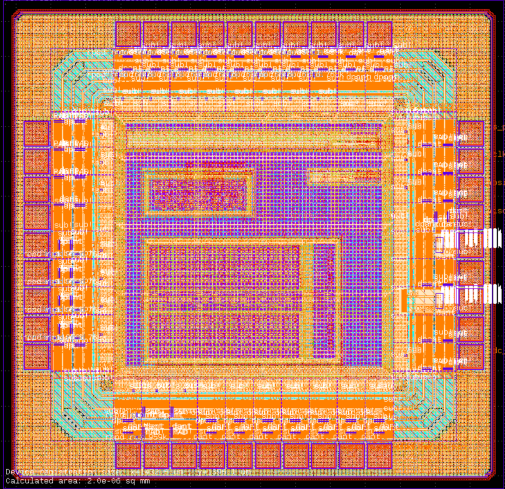
\includegraphics[width=\linewidth]{fig/layout_capture.png}
\caption{Layout (KLayout capture of the submitted GDS).}
\end{subfigure}\hfill
\begin{subfigure}{0.48\textwidth}\centering
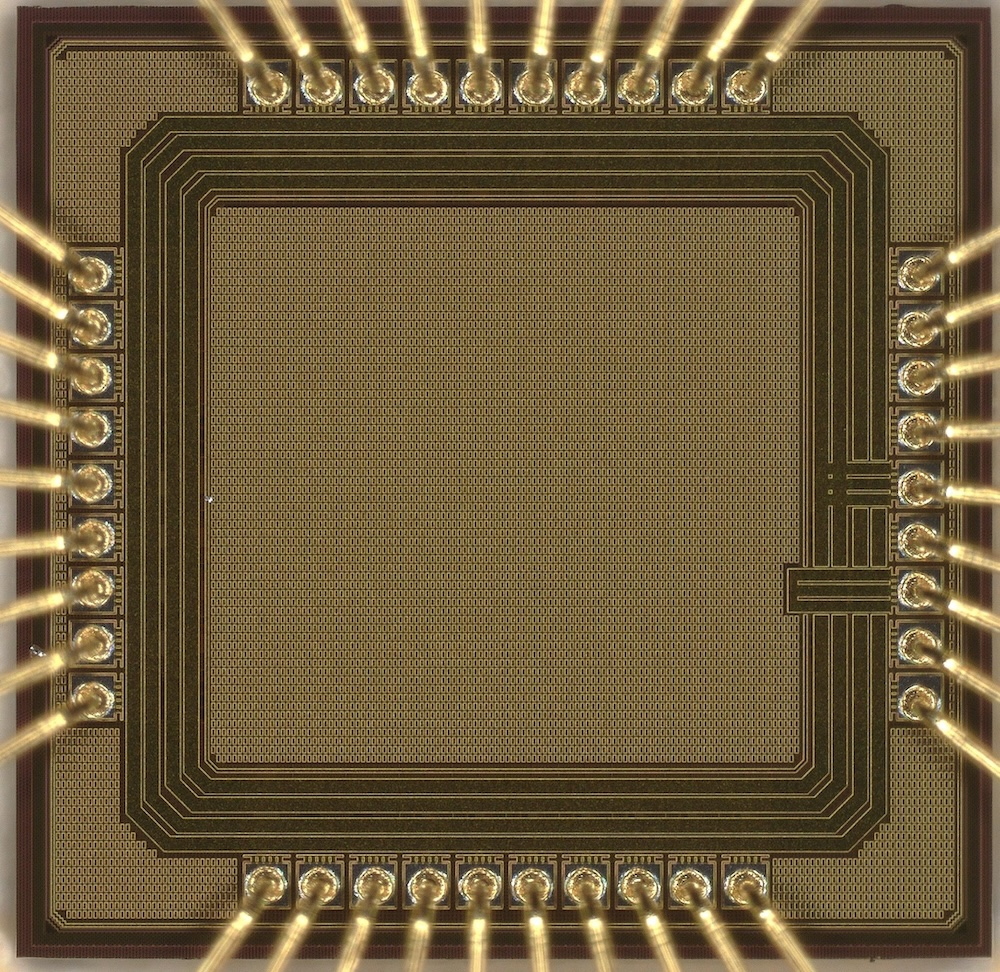
\includegraphics[width=\linewidth]{fig/die_photo.jpg}
\caption{Die photograph, bonded in the QFN48 package.}
\end{subfigure}
\caption{ASICONE. In the photograph the metal fill hides the circuits; the 38 bond wires (10 on the
top and bottom edges, 9 on the sides) are visible, and so is the seal ring.}
\label{fig:die}
\end{figure}

\subsection{Pinout}
The die is bonded in a QFN48 (\SI{0.5}{mm} pitch); 10 package pins are left open.
Table~\ref{tab:pinout} is the pinout as connected on the adapter board (Section~\ref{sec:board}).
\begin{figure}[H]\centering
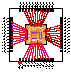
\includegraphics[width=0.55\textwidth]{fig/qfn48_bonding.pdf}
\caption{Bonding diagram (\texttt{QFN48.svg}).}
\end{figure}
\begin{table}[H]\centering\scriptsize
\begin{tabular}{rlll@{\hspace{2em}}rlll}
\toprule
Pin & Signal & Pad cell & Board net & Pin & Signal & Pad cell & Board net \\
\midrule
2 & AVDD & IOPadAnalog & \texttt{adc\_vdd} (JP5) & 26 & RO\_13\_Vout & IOPadOut16mA & \texttt{ro\_13\_vout} \\
3 & adc\_rst & IOPadIn & \texttt{adc\_rst} & 27 & RO\_101\_Vout & IOPadOut16mA & \texttt{ro\_101\_vout} \\
4 & adc\_clk & IOPadIn & \texttt{adc\_clk} & 28 & RO2VDD & IOPadAnalog & \texttt{ro2\_vdd} (JP4) \\
5--9 & adc\_result[0..4] & IOPadOut16mA & \texttt{adc\_result\_0..4} & 29 & ROVDD & IOPadAnalog & \texttt{ro\_vdd} (JP3) \\
10 & adc\_valid & IOPadOut16mA & \texttt{adc\_valid} & 30 & RO\_13\_extra\_load & IOPadAnalog & \texttt{ro\_13\_ex} \\
11 & adc\_sample & IOPadOut16mA & \texttt{adc\_sample} & 31 & RO\_13\_Drain\_Sense & IOPadAnalog & \texttt{ro\_13\_ds} \\
14 & adc\_go & IOPadIn & \texttt{adc\_go} & 32 & RO\_13\_Drain\_Force & IOPadAnalog & \texttt{ro\_13\_df} \\
15 & VSS & IOPadVssExt & GND & 33 & RO\_101\_extra\_load & IOPadAnalog & \texttt{ro\_101\_ex} \\
16 & VDD & IOPadVddExt & \texttt{vdd1p2} (JP2) & 34 & RO\_101\_Drain\_Sense & IOPadAnalog & \texttt{ro\_101\_ds} \\
17 & VSSIO & IOPadIOVss & GND & 35 & RO\_101\_Drain\_Force & IOPadAnalog & \texttt{ro\_101\_df} \\
18 & VDDIO & IOPadIOVdd & \texttt{vdd3p3} (JP1) & 38 & RO\_13\_DUT\_gate & IOPadIn & \texttt{ro\_13\_gate} \\
19 & miso & IOPadOut16mA & \texttt{miso} & 39 & RO\_101\_DUT\_gate & IOPadIn & \texttt{ro\_101\_gate} \\
20 & mosi & IOPadIn & \texttt{mosi} & 40 & RO\_RST\_B & IOPadIn & \texttt{ro\_rstb} \\
21 & sclk & IOPadIn & \texttt{sclk} & 41 & VSS (RO) & IOPadVssExt & GND \\
22 & cs & IOPadIn & \texttt{cs} & 42 & adc\_vip & IOPadAnalog & \texttt{adc\_vip} (JP9) \\
 & & & & 43 & adc\_vin & IOPadAnalog & \texttt{adc\_vin} (JP10) \\
 & & & & 44 & adc\_vrefn & IOPadAnalog & \texttt{adc\_vrefn} (JP7) \\
 & & & & 45 & adc\_vrefp & IOPadAnalog & \texttt{adc\_vrefp} (JP6) \\
 & & & & 46 & VSS (ADC) & IOPadVssExt & GND \\
\bottomrule
\end{tabular}
\caption{Pinout. Open package pins: 1, 12, 13, 23, 24, 25, 36, 37, 47, 48. Analog signals connect to
the core through the \texttt{padres} terminal of \texttt{sg13g2\_IOPadAnalog} (secondary protection
resistor of about \SI{587}{\ohm} and ESD diodes); the ring supplies use the direct \texttt{pad} terminal.}
\label{tab:pinout}
\end{table}

%=====================================================================
\section{Block design}
\subsection{Custom standard cells}
Every digital cell on the chip is custom. Two libraries were drawn for this tapeout:
\begin{itemize}
  \item \texttt{sg13g2} (\texttt{lib/}): 86 cells, 18 tracks (\SI{6.12}{\micro m} rows on a
        \SI{0.34}{\micro m} site), used by the SPI and the top level;
  \item \texttt{sg13g2f} (\nolinkurl{saradc_auto/cells/}): 77 floating-body variants used inside the ADC,
        plus the analog cells \texttt{SARADC\_CELL\_INVX16\_ASCAP} (unit capacitor) and
        \texttt{SARADC\_CELL\_INVX0\_ASSW} (switch).
\end{itemize}
The 18-track height is generous and the cells are not optimized: the standard-cell generator was
still in development. The Liberty timing was \emph{not} characterized in SG13G2; it was adapted from
\texttt{sky130}, because the PDK had no parasitic extraction to characterize the layouts with. Timing
of the digital blocks is therefore nominal only; at the clock rates used (\SI{10}{MHz} for the ADC, a few
MHz for the SPI) this was never a limitation.

\subsection{SAR ADC}
\label{sec:adc_design}
\paragraph{Architecture.} The ADC is a fully differential, top-plate-sampling charge-redistribution
SAR ADC. Each side has a binary capacitive DAC of $2^5$ units (bits of 1, 2, 4, 8, 16 units plus a
dummy) between a switched plate (VSH: input, VREFH or VREFL) and a floating top plate (FL) that feeds
the comparator inputs VOUTH/VOUTL. The unit capacitor is the gate of a group of MOS transistors
(\SI{67.8}{fF} per unit with FL floating); there are 720 unit-capacitor cells and 1452 switch cells. The
comparator is a dynamic latch built from \texttt{sg13g2f} cells; the SAR logic
(\texttt{sar\_logic\_wreset.v}) is synthesized. A conversion takes $N + 2 = 7$ clocks: sampling, five
bit decisions and the result. Interface: \texttt{CLK}, \texttt{RST} (active high), \texttt{GO} (start
conversions), \texttt{SAMPLE}, \texttt{VALID} and \texttt{RESULT[4:0]}.

\paragraph{Generator and flow.} \texttt{saradc\_auto} produces the ADC from RTL: Yosys synthesizes the
analog netlist (capacitors and switches as cells) and the logic; OpenROAD places the DAC array with a
scripted pattern (a ``circle'' pattern with Metal5/TopMetal1 bridges for bits 1 and 3), routes the special
nets (plates, references, top plates) with custom Tcl, and routes the rest with the detailed router. The
taped-out version used the flat flow now kept as \texttt{pnr\_legacy/}. Macro size
\SI{566.44}{\micro m} $\times$ \SI{361.08}{\micro m}, 24\,198 transistors. The taped-out netlists, DEF,
GDS and reports are archived in the release \texttt{tapeout-T594} of \texttt{saradc\_auto}
(\url{https://github.com/ckdur/saradc_auto/releases/tag/tapeout-T594}); its \texttt{SARADC.gds} is
identical, layer by layer, to the \texttt{SARADC} cell of the submitted chip GDS.

\paragraph{Design-time simulation.} Before tapeout the ADC was verified at schematic level with
ngspice and Xyce at \SI{1.8}{V}: transient conversions (only a few samples were possible at the
time with the analog netlist), multi-frequency tests, a capacitor-linearity test and a switch-charge
test (commits of 30 August to 5 September 2025). No layout parasitics were available
(Section~\ref{sec:pex}).

\subsection{Ring oscillators}
Each ring (\texttt{top\_13}, \texttt{top\_101}) has 13 or 101 inverting stages of \texttt{lv} MOS
($L = \SI{0.45}{\micro m}$, $W_p/W_n = 4\times\SI{3.4}{\micro m}/4\times\SI{1.3}{\micro m}$), a 5-flop
ripple divider ($\div 32$, reset by \texttt{RO\_RST\_B}) and a \SI{16}{mA} output pad. Three stages are
special: \texttt{rovcel3} closes or opens the ring (header/footer on \texttt{n\_RO\_control},
\texttt{RO\_control}) and, with the ring open, connects \texttt{DUT\_gate} to the DUT input;
\texttt{rovcel1} is the DUT, with a PMOS header (\texttt{DUT\_Header}) and NMOS footer
(\texttt{DUT\_Footer}), whose output (\texttt{extra\_load}) goes straight to an analog pad and, with the
ring open, to \texttt{Drain\_Force}/\texttt{Drain\_Sense} through transmission gates; \texttt{rovcel4}
has a PMOS header on \texttt{n\_RO\_control}. RO101 is supplied from ROVDD, RO13 from RO2VDD; both share
the core VSS. The control bits come from SPI register 0 (RO101, \texttt{R[3:0]}) and register 1 (RO13,
\texttt{R[11:8]}): bit 0 \texttt{n\_RO\_control}, 1 \texttt{RO\_control}, 2 \texttt{DUT\_Footer},
3 \texttt{DUT\_Header}; oscillation is \texttt{0x06}. The ROs were integrated last, on
12 September 2025, the day of the final submission.

\subsection{SPI}
\nolinkurl{digital/rtl/spix/spi.v}, parameters \texttt{registers=8}, \texttt{inputs=6}, \texttt{sword=8},
\texttt{syncing=0} (one-hot shift counter), \texttt{addressing=1} (multiplexer read). Frame, sampled on
the rising SCLK with CS low: write bit, read bit, \texttt{addr[2:0]}, \texttt{data[7:0]}, then, for a
read, 8 bits shifted out on MISO. The register is written on the 14th edge; the bit counter only
restarts on an SCLK edge with CS high. Synthesized to 108 \texttt{DFCNQD1} flops, 91 \texttt{MUX2D1}
and about 140 other gates; macro \SI{311.6}{\micro m} $\times$ \SI{128.4}{\micro m}. Read map: register 0 = ADC result,
1 = \{sample, valid\}, 2/3 = constant \texttt{0xAA}/\texttt{0x55}, 4/5 = write registers 0/1 (echo).
The SPI reset is the \texttt{adc\_rst} pad (Section~\ref{sec:spi}).

%=====================================================================
\section{Design flow and tapeout sequence}
\label{sec:tapeout}
\subsection{Flow}
The flow is custom (no OpenROAD-flow-scripts), organized per block as
\texttt{syn} (Yosys) $\to$ \texttt{pnr} (OpenROAD) $\to$ \texttt{signoff} (KLayout GDS merge, fill,
DRC, LVS), and at the top as \texttt{padring} (the \texttt{padring} tool, \texttt{.cfg} with corners,
pads, bond pads and fillers) $\to$ \texttt{pnr} (macro placement, power grid, routing) $\to$
\texttt{signoff}. Versions used for the final sign-off:
\begin{center}\small
\begin{tabular}{ll}
\toprule
IHP-Open-PDK & \texttt{6bda9f1cd9ae7108571041d9bd0f03a5a94f731f} \\
OpenROAD & \texttt{59ef9a94573c0a6799d32e2dfc9fc7a93feeb30f} \\
Yosys & \texttt{4581f75b03a25b615a9715516854c424b580f7ab} (0.49 for the SPI netlist) \\
KLayout & 0.30.2 (\texttt{d1dc885235bf571eac7270d6dccca820a019b4b1}) \\
ngspice & 44.2 \\
OpenVAF-Reloaded & \texttt{802bce21ac44833b52c010cb90d37e0d6fddd4ac} \\
\bottomrule
\end{tabular}
\end{center}

\subsection{Timeline}
Reconstructed from the commit history of \texttt{asicone\_sg13g2}, of the submission fork
\texttt{TO\_Sep2025} and of the sign-off logs (all times JST).
\begin{longtable}{p{0.15\linewidth}p{0.79\linewidth}}
\toprule
Date & Step \\
\midrule
\endhead
\multicolumn{2}{l}{\textit{Preparation (May--July 2025)}} \\
2025-05-12 & First commit: digital flow for the custom cells. \\
05-16 -- 05-19 & First OpenROAD PnR of a digital block, up to CTS. \\
06-16 -- 06-30 & First full PnR and sign-off of the digital block; DRC working, LVS not yet. \\
07-21 & Synthesis fixed, first LVS-clean digital block; fillers added and first pad ring generated;
  first top-level PnR draft. \\
07-23 -- 07-29 & Pad-ring configuration, first OpenROAD script for the chip; the ADC brought into the repository. \\
\multicolumn{2}{l}{\textit{ADC physical design (August 2025)}} \\
08-05 -- 08-08 & First synthesis of the ADC, placement, blockages; first ADC with all routes but no connections. \\
08-12 & IHP opens the \texttt{TO\_Sep2025} repository (rules: \SI{2}{mm^2} including seal ring, registration
  1 September, DRC-clean GDS by 14 September, no changes afterwards). \\
08-14 & Via generation for the custom routes. \\
08-17 -- 08-19 & Joining of the ADC routes, power stripes, first placement and CTS of the chip. \\
08-20 & First complete PnR; final pad-ring and seal-ring size; bond pads. Placeholder submitted to \texttt{TO\_Sep2025}. \\
08-21 -- 08-22 & Assets reorganized, LEF fixes, comparator routes; full chip flow complete (unverified), better detailed routing. \\
\multicolumn{2}{l}{\textit{DRC and LVS closure (23--28 August)}} \\
08-23 & DRC fixes in the metal stack and in the standard cells. \\
08-24 & ADC DRC reduced from about 5000 to 20 violations, then 38 left at the top. \\
08-25 & ADC DRC clean; LVS debugging, cells rejected by LVS removed. \\
08-26 & LVS clean on the SARADC; libraries renamed and separated (\texttt{sg13g2}/\texttt{sg13g2f}); full chip assembled. \\
08-27 & Manufacturing-grid fixes, DRC fixes, custom LVS deck support; die size corrected for the
  seal-ring-to-passivation rule (\texttt{TO\_Sep2025}). \\
08-28 & I/O cells customized for LVS (missing \texttt{PolyRes} recognition layer added); \texttt{ptap1}
  ignored in a custom deck; \textbf{full-chip LVS pass}. \\
\multicolumn{2}{l}{\textit{Verification and submission (29 August -- 14 September)}} \\
08-29 -- 08-31 & ADC testbenches; submission metadata; simulation folder of the submission. \\
09-01 & Registration deadline. ADC simulations ported to Xyce; SAR logic changed to flops with reset for the result. \\
09-02 -- 09-05 & Multi-frequency, capacitor-linearity and switch-charge simulations of the ADC. \\
09-09 & Correction of the \texttt{sg13g2} library. \\
09-12 01:13 & First integration of the ring oscillators into the chip. \\
09-12 10:18 & First sign-off of the chip with the ROs. \\
09-12 21:18 & Final sign-off runs on \texttt{asicone\_202508.fill.gds}: LVS (KLayout 0.30.2, flat, custom deck) ``Netlists match'' at 22:53 (\SI{95}{min}); full DRC with antenna and density at 23:15 (\SI{117}{min}). \\
09-12 23:40 & Final upload to \texttt{TO\_Sep2025} (\texttt{asicone\_202509}): GDS, DRC, LVS, simulation and digital data, metadata. \\
09-12 23:49 & ``Everything ready'' in \texttt{asicone\_sg13g2}. \\
09-14 & Shuttle deadline. \\
\multicolumn{2}{l}{\textit{After the tapeout}} \\
09-15 -- 10-03 & Submodule fixes, pad-ring tool included, license and README; the ADC moved to its own repository (\texttt{saradc\_auto}). \\
2025-12 -- 2026-01 & Repositories moved to GitLab, \texttt{run.sh} demo, fixes for newer OpenROAD. \\
2026-05-08 & QFN48 bonding diagram. \\
2026-08-17 & Die photograph of the packaged chip. \\
2026-08-28 -- 09-24 & Adapter board designed (first commit; fabrication files on 09-24) (\texttt{IHP130\_ASICONE\_ADP\_QFN48\_0p5Q\_Adapter}). \\
2026-09-12 -- 09-25 & RISCVConsole SoC ported to the ULX3S (SD boot, extra SPIs, external \SI{10}{MHz} clock). \\
2026-10-01 -- 10-19 & First ADC conversions on the bench, fast sampling firmware. \\
2026-10-22 & ADC sweep with the MSO20 (data set \texttt{sweep\_20261022}). \\
2026-10-24 -- 10-25 & ADC compared with schematic and post-layout simulation. \\
2026-10-29 -- 10-30 & Ring-oscillator measurement (\texttt{ro\_20261029}) and post-layout comparison. \\
\bottomrule
\end{longtable}
The critical path was clear: the ADC went from its first routed layout (8 August) to DRC clean
(25 August) and LVS clean (26 August) in under three weeks, leaving two weeks for the full-chip
verification, the simulations and the RO integration, and no time for any post-layout iteration.

\subsection{Sign-off results and deviations}
\begin{itemize}
  \item \textbf{DRC}: the full KLayout deck (flat, antenna, density) reports 52 violations, all in the
        IHP I/O cells: 26 \texttt{Sdiod.d} and 26 \texttt{Sdiod.e}. They were accepted; the I/O
        works on silicon. All the designed blocks are DRC clean.
  \item \textbf{LVS}: ``Netlists match'' with a custom deck: \texttt{ptap1} is ignored entirely (the
        extractor turned substrate taps into diodes, which only match if each tap is a separate diode,
        and merged taps in the layout create a single diode), and a \texttt{PolyRes} layer missing in some
        I/O sub-cells was added so that the \texttt{rppd} resistors are recognized.
  \item Capacitors were attached to some transistors of the netlist for simulator convergence.
  \item No parasitic extraction (Section~\ref{sec:pex}) and no timing characterization in SG13G2.
  \item No gate-level or RTL regression of the SPI read path: its testbench (\texttt{spi\_tb.v}) still
        used an old port name (\texttt{DOUT}) and no longer elaborated against the taped-out
        \texttt{spi.v}. DRC and LVS only check that the layout implements the netlist; they cannot
        catch a logic error in the RTL (Section~\ref{sec:spi}).
\end{itemize}

\subsection{Parasitic extraction: not available at tapeout}
\label{sec:pex}
At tapeout the SG13G2 PDK had no parasitic-extraction rules, so neither the ADC nor the ROs could be
simulated with their layout. After the measurements several routes were tried:
Magic 8.3.623 (capacitances about $100\times$ too large, and Netgen cannot compare the netlist),
and KLayout-PEX~\cite{kpex} on the whole flat layout (single-threaded 2.5D engine; runs of 4, 12, 10 and
\SI{16}{h} never finished). What finally worked is a \emph{split} extraction: the layout is cut into
small windows along fillers and taps (81 for the ADC), each window is extracted with KLayout-PEX 0.3.12
(2.5D, coupling capacitances, \emph{no resistance}) after the PDK LVS deck with its unconditional
\texttt{purge} disabled, and the windows are stitched by net name. The stitched ADC netlist has the 24\,198
transistors and 68\,519 capacitors and matches the schematic on all 572 named nets. The RO cells were
extracted the same way from the fabricated GDS. These are the post-layout results quoted in this
report; they were not available when the chip was designed.

%=====================================================================
\section{Measurement environment}
\label{sec:bench}
\begin{figure}[H]\centering
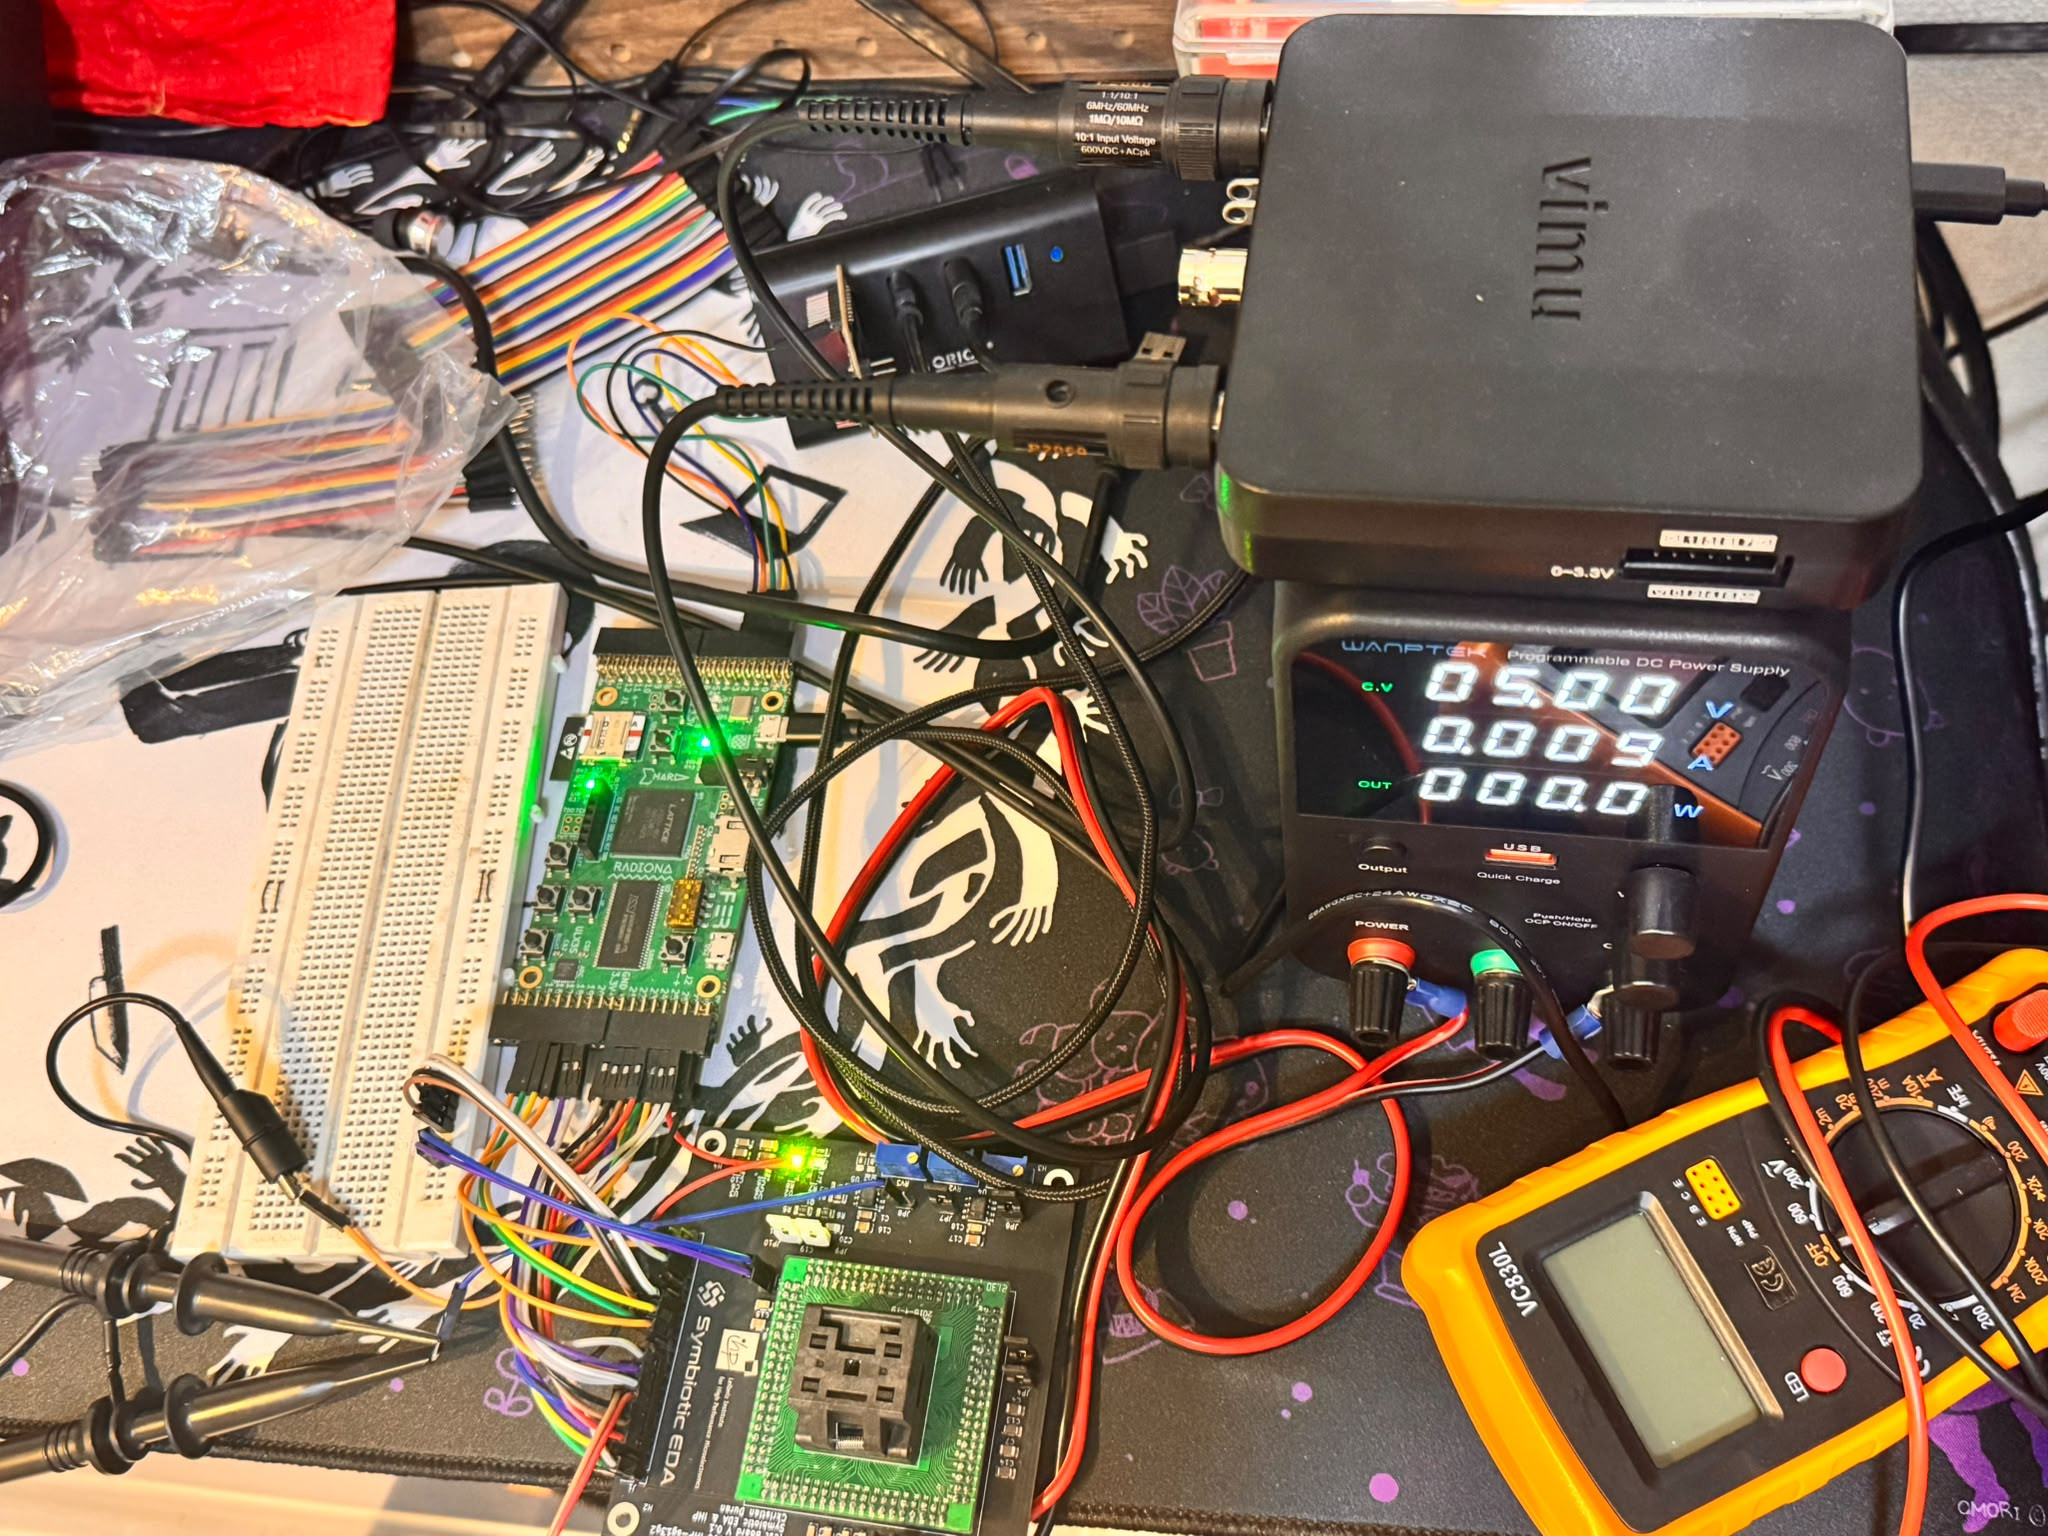
\includegraphics[width=0.95\textwidth]{measurement_setup.jpeg}
\caption{The bench. Bottom centre: the adapter board with the chip in a QFN48 clamshell socket;
left of it the ULX3S FPGA board (Lattice ECP5) wired to the adapter header J1 with jumper wires and a
breadboard; top right: the Vimu MSO20 oscilloscope/DDS with its probes; right: a Wanptek programmable DC
supply and a VC830L multimeter (used for the reference and supply voltages); a powered USB hub connects
the instruments, the JTAG adapter and the FPGA to the host PC.}
\label{fig:bench_photo}
\end{figure}

\subsection{Equipment and signal chain}
The bench is kept in two repositories: the adapter board in \texttt{pcbs}
(\url{https://gitlab.symbioticeda.com/ckdur.iso/pcbs}), and the FPGA SoC with the bench scripts and
report generators in \texttt{RISCVConsole} (\url{https://github.com/ckdur/RISCVConsole}, branch
\texttt{adc-sim-comparison}, commit \texttt{c32ae7a}); Section~\ref{sec:repro} describes how to repeat the
measurements.
\begin{table}[H]\centering\small
\begin{tabular}{lp{0.66\linewidth}}
\toprule
Device under test & ASICONE in a QFN48 clamshell socket on the adapter board \\
Adapter board & \texttt{IHP130\_ASICONE\_ADP\_QFN48\_0p5Q\_Adapter} (Section~\ref{sec:board}) \\
Digital host & ULX3S, Lattice ECP5-85F, RISCVConsole SoC: RV64IMAC Rocket core, buses at \SI{50}{MHz};
  ADCFIFO (\texttt{0x64003000}), SiFive SPI (\texttt{0x64002000}), \texttt{rocounter} (\texttt{0x64005000}) \\
Firmware & RISCVConsoleCode, branch \texttt{ihp} (\texttt{src/adc.c}, \texttt{src/ro.c}) \\
Signal source & Vimu MSO20BL, DDS channel 1, driven by VmMsoOpenSDK (\nolinkurl{software/mso/mso_dds}) \\
Voltage reference & MSO20 channel 1 on the DDS output, DC, \SI{\pm 1}{V} range, 8192 samples per capture \\
ADC clock & \SI{10}{MHz} from the FPGA PLL; 7 clocks per conversion, $f_s = \SI{1.4286}{MS/s}$ \\
Frequency counting & \texttt{rocounter}: 3-flop synchronizer and edge counter, gate of \num{50000000}
  bus cycles (\SI{1}{s}, \SI{1}{Hz} resolution at the pad, \SI{32}{Hz} at the ring) or \SI{100}{ms} \\
Debug and data & FT232H JTAG (OpenOCD) for boot and buffer dump; ULX3S USB UART at \SI{115200}{baud} \\
DC & Multimeter VC830L; bench supply (Wanptek) available for supply sweeps through JP3/JP4 \\
\bottomrule
\end{tabular}
\caption{Equipment.}
\end{table}

\begin{figure}[H]\centering
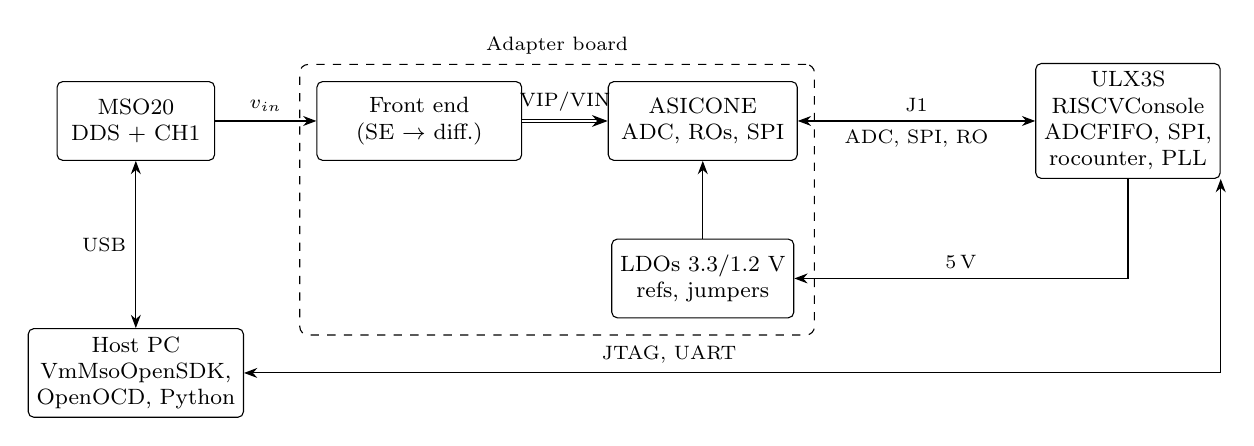
\begin{tikzpicture}[font=\footnotesize, >=Stealth,
    blk/.style={draw, rounded corners=2pt, align=center, minimum height=10mm, minimum width=20mm, inner sep=3pt, fill=white},
    grp/.style={draw, dashed, rounded corners=3pt, inner sep=6pt},
    lbl/.style={font=\scriptsize, align=center}]
  \node[blk] (dds) at (0,0) {MSO20\\DDS + CH1};
  \node[blk] (host) at (0,-3.2) {Host PC\\VmMsoOpenSDK,\\OpenOCD, Python};
  \node[blk, minimum width=26mm] (fe) at (3.6,0) {Front end\\(SE $\to$ diff.)};
  \node[blk, minimum width=24mm] (chip) at (7.2,0) {ASICONE\\ADC, ROs, SPI};
  \node[blk] (ldo) at (7.2,-2.0) {LDOs 3.3/1.2 V\\refs, jumpers};
  \node[grp, fit=(fe)(chip)(ldo)] (adp) {};
  \node[lbl, anchor=south] at (adp.north) {Adapter board};
  \node[blk] (fpga) at (12.6,0) {ULX3S\\RISCVConsole\\ADCFIFO, SPI,\\rocounter, PLL};
  \draw[->] (dds) -- node[lbl, above]{$v_{in}$} (fe);
  \draw[->, double] (fe) -- node[lbl, above]{VIP/VIN} (chip);
  \draw[<->] (chip) -- node[lbl, above]{J1}node[lbl, below]{ADC, SPI, RO} (fpga);
  \draw[->] (ldo) -- (chip);
  \draw[->] (fpga.south) |- node[lbl, pos=0.75, above]{\SI{5}{V}} (ldo.east);
  \draw[<->] (host) -- node[lbl, left]{USB} (dds);
  \draw[<->] (host.east) -- ++(9.0,0) node[lbl, above, pos=0.6]{JTAG, UART} -| (fpga.south east);
\end{tikzpicture}
\caption{Signal chain of the bench.}
\end{figure}

\subsection{Adapter board}
\label{sec:board}
A two-layer \SI{85.5}{mm} $\times$ \SI{85.5}{mm} board (KiCad, \nolinkurl{pcbs/IHP130_ASICONE_ADP_QFN48_0p5Q_Adapter}
in \url{https://gitlab.symbioticeda.com/ckdur.iso/pcbs}, assembled from the JLCPCB BOM/CPL files) that plugs into the ULX3S 2$\times$20 header and carries
everything the chip needs. All passives are 1206.
\begin{table}[H]\centering\small
\begin{tabular}{llp{0.5\linewidth}}
\toprule
Ref. & Part & Function \\
\midrule
U1 & QFN48 socket & ASICONE \\
U2 & TLV75533PDBV & \SI{3.3}{V} LDO from the \SI{5}{V} of J1: op-amps and chip I/O (VDDIO via JP1) \\
U3 & TLV75512PDBV & \SI{1.2}{V} LDO: core (JP2), ADC (JP5), ROVDD (JP3), RO2VDD (JP4), references, front-end divider \\
U4 & LMV358 & Buffers of VREFP (U4A, JP6) and VREFN (U4B, JP7), set by RV1/RV2 \\
U5 & LMV358 & Single-ended to differential front end (SBOA216~\cite{sboa216}) \\
RV1--RV3 & \SI{10}{k\ohm} Bourns 3296W & VREFP, VREFN, and a DC input (RV3, through JP8) \\
R1, R2 & \SI{10}{k\ohm} & \SI{0.6}{V} common-mode divider \\
R3, R4 & \SI{1}{k\ohm} & Gain resistors of the inverting leg (U5B) \\
R5, R6 & \SI{47.5}{\ohm} & Isolation resistors to the ADC inputs \\
C19 / C20, C21 & \SI{1.2}{nF} / \SI{120}{pF} & Differential / common-mode charge reservoir at VIP/VIN \\
C1--C18 & \SI{10}{\micro F} + \SI{100}{nF} & Decoupling of every supply pin \\
Q1, Q2, D1, D2, R7, R8 & 2N7002, LED, \SI{220}{\ohm} & ``\SI{1.2}{V}'' and ``\SI{3.3}{V}'' power indicators (MOSFET gate on the LDO output) \\
JP1--JP10 & 2-pin jumpers & Supply, reference and input selection; current measurement points \\
J1 & 2$\times$20 header & ULX3S connection \\
\bottomrule
\end{tabular}
\caption{Adapter board components.}
\end{table}

\paragraph{Front end.} U5A buffers the input ($v_p = v_{in}$); U5B is a difference amplifier with
R3/R4 referenced to the \SI{0.6}{V} of R1/R2 ($v_n = \SI{1.2}{V} - v_{in}$), so the ADC sees
$v_d = 2(v_{in} - \SI{0.6}{V})$ at a \SI{0.6}{V} common mode. R5/R6 with C19--C21 form a differential pole at
\SI{1.33}{MHz} and a common-mode pole at \SI{28}{MHz}. With VREFP/VREFN = \SI{0.8}{V}/\SI{0.4}{V} the
ideal LSB is \SI{25}{mV} differential, \SI{12.5}{mV} at the board input.

\paragraph{Header J1.} Pins 1--17: \texttt{adc\_go} (1), \texttt{miso} (2), \texttt{adc\_sample} (3),
\texttt{mosi} (4), \texttt{adc\_valid} (5), \texttt{sclk} (6), \texttt{adc\_result\_4..0} (7, 9, 13, 14, 15),
\texttt{cs} (8), \SI{5}{V} (11), GND (12, 30), \texttt{adc\_clk} (16), \texttt{adc\_rst} (17). RO signals:
\texttt{ro\_rstb} (23), \texttt{ro\_101\_gate} (24), \texttt{ro\_13\_gate} (25), \texttt{ro\_101\_df/ds/ex}
(26/27/28), \texttt{ro\_13\_df/ds/ex} (31/32/33), \texttt{ro\_101\_vout} (35), \texttt{ro\_13\_vout} (36).

\paragraph{Known limitations of the board.} (1) The LMV358 (GBW about \SI{1.4}{MHz} fitted, slew rate about
\SI{1}{V/\micro s}) limits the front end above \SI{100}{kHz}, and its two legs have different bandwidths
(unity gain vs.\ noise gain 2), which turns signal into common mode. (2) The references have no
decoupling capacitor at the chip pins. (3) The analog RO pins (\texttt{df}, \texttt{ds}, \texttt{ex})
go to J1 directly and must never see the \SI{3.3}{V} of the FPGA. A revised front end (fully differential
amplifier, decoupled references) is proposed in \nolinkurl{RISCVConsole/software/mso/pcbfix}.

%=====================================================================
\section{SAR ADC measurement}
\label{sec:adc}
Conditions: VDD = AVDD = \SI{1.2}{V}, VREFP/VREFN = \SI{0.8}{V}/\SI{0.4}{V} (multimeter), input common mode
\SI{0.6}{V}, \SI{10}{MHz} clock, $f_s = \SI{1.4286}{MS/s}$, 65\,536 samples per record, room temperature.
Static linearity by the code-density test of IEEE~1241~\cite{ieee1241} with a \SI{218}{Hz} triangle
overdriving both ends; dynamic performance with coherent sines (odd prime number of periods) and the
four-parameter fit of IEEE~1057~\cite{ieee1057}. All voltages are single-ended at the board input. The
full analysis is in \nolinkurl{RISCVConsole/software/mso/results/sweep_20261022/report/report.pdf}.

\subsection{Static linearity}
\begin{table}[H]\centering\small
\begin{tabular}{ll}
\toprule
Input range (first to last transition) & \SIrange{0.3719}{0.7696}{V} (ideal \SIrange{0.4125}{0.7875}{V}) \\
LSB & \SI{13.26}{mV} (ideal \SI{12.50}{mV}; gain error \SI{6.1}{\percent}) \\
Offset & \SI{-29}{mV} (\num{-2.2} LSB), board and comparator \\
DNL & \numrange{-0.80}{0.67} LSB \\
INL (end point) & \numrange{-0.87}{0.99} LSB, \SI{0.51}{LSB} rms \\
Missing codes & none; monotonic \\
\bottomrule
\end{tabular}
\end{table}
\begin{figure}[H]\centering
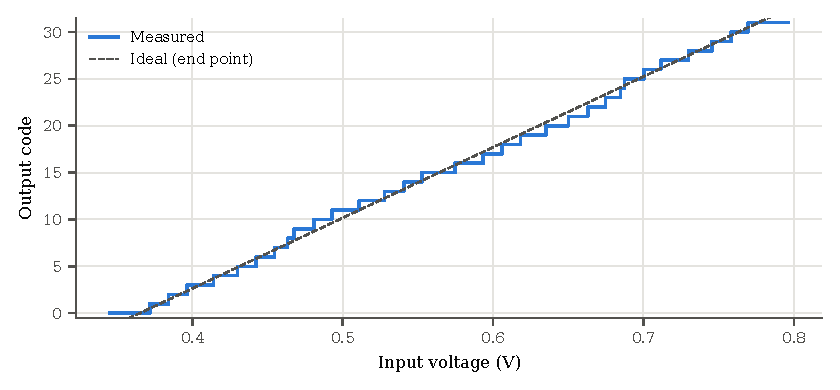
\includegraphics[width=0.75\textwidth]{fig/adc_transfer.pdf}\\
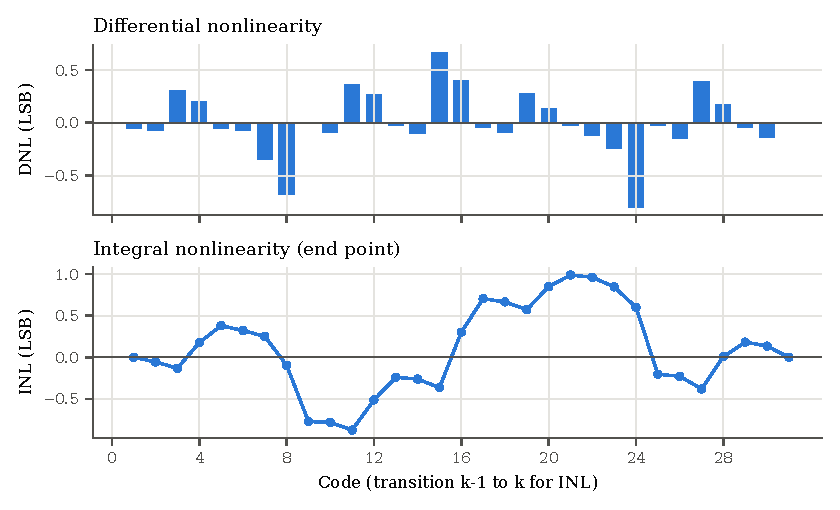
\includegraphics[width=0.75\textwidth]{fig/adc_dnl_inl.pdf}
\caption{Transfer characteristic and DNL/INL from the histogram test.}
\end{figure}
The DNL repeats every 8 codes and the INL jumps at codes 8, 16 and 24: the signature of wrong binary
weights in the DAC. A least-squares fit of the transition levels to the bits gives:
\begin{table}[H]\centering\small
\begin{tabular}{lccccc}
\toprule
Bit & 0 & 1 & 2 & 3 & 4 \\
\midrule
Ideal weight (LSB) & 1 & 2 & 4 & 8 & 16 \\
Measured weight & 0.92 & 1.89 & 4.27 & 7.33 & 16.55 \\
Measured error (\%) & $-7.8$ & $-5.7$ & $+6.7$ & $-8.4$ & $+3.5$ \\
Schematic simulation (\%) & $+0.0$ & $-0.1$ & $+0.0$ & $+0.0$ & $+0.0$ \\
Post-layout, taped-out GDS (\%) & $-12.5$ & $-6.8$ & $+3.3$ & $-5.2$ & $+2.3$ \\
\bottomrule
\end{tabular}
\caption{Binary weights of the DAC. After removing them, \SI{0.19}{LSB} rms of INL remain.}
\label{tab:weights}
\end{table}

\subsection{Dynamic performance}
\begin{table}[H]\centering\small
\begin{tabular}{rrrrrrrr}
\toprule
$f_{in}$ (kHz) & $A$ (LSB) & SINAD (dB) & ENOB & THD (dB) & SFDR (dB) & H2 (dBc) & H3 (dBc) \\
\midrule
1.0 & 13.29 & 24.69 & 3.81 & $-27.5$ & 32.9 & $-45.4$ & $-31.5$ \\
10.0 & 13.29 & 24.85 & 3.84 & $-27.4$ & 33.0 & $-45.1$ & $-31.4$ \\
50.0 & 13.27 & 24.73 & 3.82 & $-27.4$ & 32.4 & $-46.2$ & $-32.5$ \\
100.1 & 13.09 & 23.93 & 3.68 & $-26.0$ & 29.9 & $-43.9$ & $-34.6$ \\
200.0 & 12.80 & 23.48 & 3.61 & $-25.2$ & 29.8 & $-43.9$ & $-31.1$ \\
300.0 & 12.16 & 23.37 & 3.59 & $-25.3$ & 29.9 & $-39.0$ & $-33.2$ \\
500.0 & 9.89 & 22.29 & 3.41 & $-24.3$ & 30.7 & $-27.5$ & $-32.2$ \\
650.0 & 6.66 & 20.30 & 3.08 & $-22.9$ & 27.6 & $-24.3$ & $-29.9$ \\
\bottomrule
\end{tabular}
\caption{Sine sweep (input \SI{360}{mV} peak-to-peak DDS setting, \SI{565}{mV} bias). An ideal 5-bit
quantizer at the low-frequency amplitude gives \SI{30.2}{dB} (4.72 bits).}
\end{table}
\begin{figure}[H]\centering
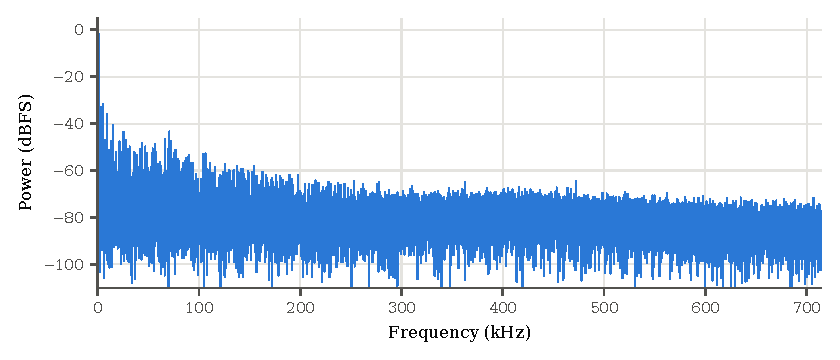
\includegraphics[width=0.75\textwidth]{fig/adc_spectrum_low.pdf}
\caption{Spectrum at \SI{1}{kHz}.}
\end{figure}
Below \SI{50}{kHz} the measured SINAD equals, within \SI{0.3}{dB}, the SINAD predicted from the ramp
transfer alone: the ENOB of 3.81 bits is entirely the static nonlinearity, i.e.\ the DAC weights. Above
\SI{100}{kHz} the board front end takes over: the amplitude falls to half at \SI{650}{kHz}, the common-mode
ripple reaches \SI{47}{\percent} of the signal and the op-amps approach their slew limit, which produces
the rising H2.

\subsection{Comparison with simulation}
\begin{figure}[H]\centering
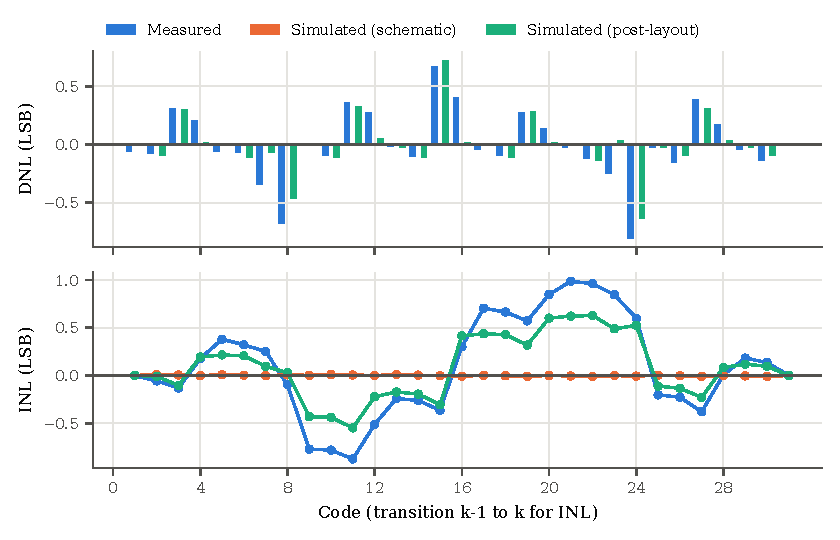
\includegraphics[width=0.75\textwidth]{fig/adc_cmp_dnl_inl.pdf}
\caption{DNL/INL: chip, schematic and post-layout simulation of the taped-out layout.}
\end{figure}
\begin{figure}[H]\centering
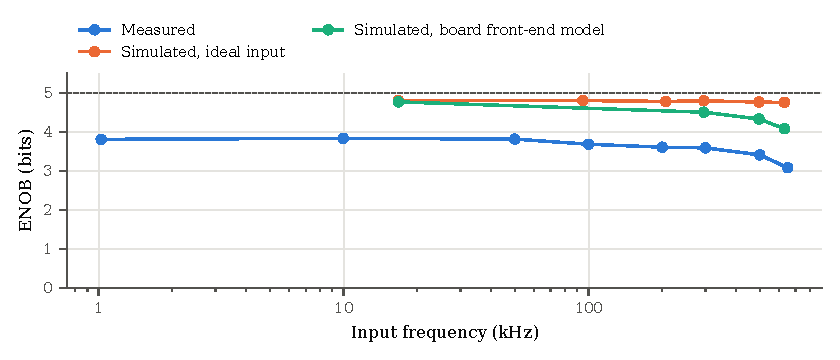
\includegraphics[width=0.75\textwidth]{fig/adc_cmp_enob.pdf}
\caption{ENOB: chip, transient simulation with ideal input, and with the front-end model of the board.}
\end{figure}
\begin{itemize}
  \item \textbf{Schematic} (ngspice-47, PSP103, TT, \SI{25}{\celsius}, board conditions): ideal --- weights
        within \SI{0.1}{\percent}, INL \SI{0.006}{LSB} rms, ENOB 4.80 at low frequency and 4.76 at
        \SI{631}{kHz}. The converter core has no dynamic loss up to Nyquist.
  \item \textbf{Post-layout} (split extraction of the taped-out GDS): weight errors with the sign of the
        measurement on all five bits, INL \SI{0.33}{LSB} rms, INL correlation 0.98 and DNL correlation 0.90
        with the chip, gain error \SI{7.1}{\percent} (measured \SI{6.1}{\percent}). Quantizing the measured
        input with the post-layout transitions gives 4.19 bits: the layout accounts for about half of the
        lost bit, and for the whole error \emph{pattern}.
  \item \textbf{With the board model}, the simulated ENOB falls by about 0.7 bits up to \SI{631}{kHz},
        the same loss as measured (3.81 $\to$ 3.08); the measured curve is about one bit below the
        simulated one at every frequency --- the static weights again.
\end{itemize}

\subsection{Why the ADC performance is poor}
\label{sec:adc_why}
The ``efficiency'' of the ADC --- how much of its 5 bits it delivers --- is low: 3.8 of the 4.7 bits an
ideal quantizer would give at the same amplitude, and less at high frequency. The causes, in order of
weight:
\begin{enumerate}
  \item \textbf{DAC plate wiring capacitance (layout).} The plates of each bit have wiring capacitance of
        the order of the unit capacitor itself (about \SI{100}{fF} per unit on VSH, 65--\SI{75}{fF} on FL),
        and part of it couples directly to the comparator inputs, differently for every bit: the bit 1/3
        bridges add about \SI{10}{\percent} of wiring capacitance; the MSB switched plate couples
        \SI{11.3}{fF} per unit to its own comparator input, the others about \SI{5}{fF}; the floating plates of
        bits 0--3 couple 7--\SI{10}{fF} per unit to the opposite input; and the two halves of the flat layout
        are not mirror images. This is fully determined by the generator's routing, not by the process.
  \item \textbf{No extraction at tapeout and no time to iterate.} Without extraction rules for SG13G2 the
        layout could only be verified for DRC and LVS. The ADC reached LVS clean 17 days before the
        deadline, and the rest of that time went into full-chip closure. The effect was invisible until
        the split extraction of October 2026.
  \item \textbf{Remaining, unexplained part} (\SI{0.20}{LSB} rms of INL; bit 0 less reduced, bit 2 larger,
        bit 3 smaller than post-layout): of the size that random unit-capacitor mismatch, the wiring
        resistance (not extracted) or the undecoupled board references can produce. A ramp with
        \SI{100}{nF} + \SI{1}{\micro F} at pins 44/45 would separate board from chip.
  \item \textbf{The board} above \SI{100}{kHz} (LMV358 front end), which is not the ADC.
\end{enumerate}
The generator has since been corrected (branch \texttt{dac-routing-fix}, \nolinkurl{docs/dac_wiring.md}): a
bridge-less nested capacitor pattern and re-assigned switch-row rails bring the per-unit plate capacitance
of all bits within a few percent and the plate-to-comparator coupling below \SI{0.5}{fF}; a hierarchical
layout with one half mirrored halves the post-layout INL (\SI{0.17}{LSB} rms, 4.52 bits). The power of the
ADC was not measured, so no figure of merit is given; the current through JP5 is the next measurement.

%=====================================================================
\section{Ring oscillator measurement}
\label{sec:ro}
Conditions: ROVDD and RO2VDD from the on-board \SI{1.2}{V} LDO through JP3/JP4, room temperature,
\texttt{df}/\texttt{ds} tied to \SI{1.2}{V}, \texttt{ex} open, \texttt{adc\_rst} held high (it is the SPI
reset). Firmware \texttt{ro\_test}, \texttt{ro\_diag}, \texttt{ro\_scan}; five runs, 132 restarts per ring
in six different ways. Full report: \nolinkurl{RISCVConsole/software/ro/results/ro_20261029/report/report.pdf}.

\subsection{Results}
\begin{table}[H]\centering\small
\begin{tabular}{lrr}
\toprule
 & RO13 & RO101 \\
\midrule
Pad, ring alone (\SI{1}{s} gate) & \SI{4.088}{MHz} & \SI{4.231}{MHz} \\
Ring frequency (pad $\times$ 32), alone & \SI{130.8}{MHz} & \SI{135.4}{MHz} \\
Change when the other ring runs & \SI{-4.0}{\percent} & \SI{+0.2}{\percent} \\
Repeatability (std.\ dev.) & \SI{0.10}{\percent} & \SI{0.11}{\percent} \\
Spread over 132 restarts & \SI{1.24}{\percent} & \SI{0.24}{\percent} \\
Duty cycle at the pad & \SI{49.6}{\percent} & \SI{49.7}{\percent} \\
\midrule
Schematic + pad, TT & \SI{223.9}{MHz} & \SI{32.3}{MHz} \\
Post-layout (wiring C), TT / SS / FF & 188.8 / 169.3 / \SI{209.8}{MHz} & 27.7 / 25.0 / \SI{30.6}{MHz} \\
Post-layout, TT, \SI{1.0}{V} & \SI{139.5}{MHz} & \SI{20.7}{MHz} \\
\midrule
Measured / post-layout TT & 0.69 & 4.88 \\
$f_{13}/f_{101}$ & \multicolumn{2}{c}{measured 0.97, predicted 6.93 (6.86--6.99 over corners)} \\
\bottomrule
\end{tabular}
\caption{Ring oscillators: bench against simulation.}
\end{table}

\paragraph{Function.} The SPI writes arrive: in the 16-value scan the rings oscillate only for
\texttt{0x06}/\texttt{0x0e} (\texttt{RO\_control}=1, \texttt{n\_RO\_control}=0, \texttt{DUT\_Footer}=1),
\texttt{RO\_RST\_B} low stops both outputs and the \SI{50}{\percent} duty cycle confirms the dividers.
Two observations do not match the design: \texttt{DUT\_Header} (bit 3) has no visible effect --- with the
header off the rings keep running (RO13 \SI{+4.5}{\percent}, RO101 \SI{-0.2}{\percent}) where the DUT
can only pull down and the ring should stop --- and with the ring open and \texttt{DUT\_gate}=1
(\texttt{0x04}, \texttt{0x0c}) RO13 shows a slow \SI{12}{kHz} oscillation at the pad.

\begin{figure}[H]\centering
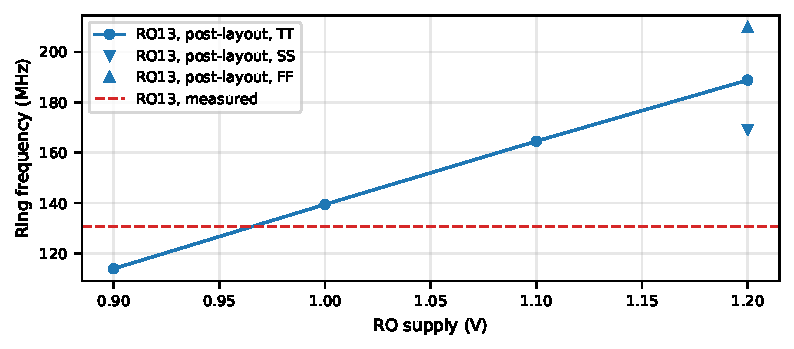
\includegraphics[width=0.7\textwidth]{fig/ro_vdd_pex.pdf}
\caption{Post-layout RO13 against its supply, and the measured frequency.}
\end{figure}

\subsection{Is the mismatch justified?}
\label{sec:ro_why}
The ADC story --- missing extraction and no time to iterate --- explains a \emph{slower} circuit,
because wiring capacitance and resistance can only lower the frequency. It explains part of RO13 and
nothing of RO101.

\paragraph{RO13: partly justified, not fully.} The extraction lowers RO13 by \SI{16}{\percent}, but the
chip is a further \SI{31}{\percent} below the post-layout TT and below the SS corner; the post-layout ring
would need about \SI{0.97}{V} to match. Candidates: (a) wiring \emph{resistance}, not extracted (the
extraction is capacitance only); in a ring of \texttt{lv} inverters with $4\times$ fingers this is
usually a few percent, not tens; (b) supply and ground drop: RO13 slows \SI{4}{\percent} when RO101 runs,
which at \SI{12}{\percent} per \SI{100}{mV} means about \SI{40}{mV} lost for the \SI{0.5}{mA} of the
other ring --- some \SI{80}{\ohm} of shared impedance, large for a board, and suggesting a shared on-chip
path (both rings return through the core VSS); a \SI{230}{mV} drop for RO13's own current would need several
hundred ohms, so the supply alone does not close the gap either; (c) the model corner, with the SS corner
already \SI{10}{\percent} faster than the chip. Each is plausible, none is measured, and together they
are at the limit of what they can explain. RO13 is therefore \emph{not yet justified}: ROVDD/RO2VDD must
be measured at the jumpers with each ring off, alone and both on, and the ring swept from a bench supply.

\paragraph{RO101: not justified by any parasitic.} RO101 runs $4.9\times$ faster than its post-layout
fundamental, \SI{37}{ps} per stage for one edge in 101 stages, which this process cannot do (RO13 shows
about \SI{290}{ps} per stage on the same chip). The measured value matches instead a ring with
about seven circulating edges: scaled by RO13's factor (0.69) the fundamental would be \SI{19.2}{MHz} and
the measurement is $7.05\times$ that --- or, equivalently, a single edge in a loop of about 14 stages,
almost RO13's 13. The numbers on the bench support ``something short'' more than ``something slow'':
$f_{13}/f_{101} = 0.97$ instead of 6.93, a duty cycle of exactly \SI{50}{\percent}, and the same frequency
after every restart, including the footer-off restart that launches a single edge. In simulation the
extracted 101-stage ring does not keep a harmonic mode: an all-zero start begins with 3 edges (4 without
wiring capacitance) that merge within \SI{0.75}{\micro s}, ending at the fundamental. The extracted cell
also has a single 101-stage loop. So either:
\begin{itemize}
  \item the chip keeps re-creating edges until about seven circulate --- the \texttt{extra\_load} node, slowed
        by its pad (\SI{587}{\ohm} and ESD capacitance), is the first suspect: a slow edge with noise can
        switch the next stage twice; or
  \item a short loop exists on silicon that is not in the extracted cell (a defect, or a path outside the
        cell); or
  \item the DUT stage is not behaving as designed, which the dead \texttt{DUT\_Header} control also
        suggests. One mechanism worth testing: the \texttt{Drain\_Force}/\texttt{Drain\_Sense} transmission
        gates are tied to \SI{1.2}{V} on the bench; any conduction through them in oscillation mode pulls the
        DUT output up independently of its header, which would explain why the header has no effect and would
        distort the DUT edge.
\end{itemize}
Note that the full-chip LVS matched with the RO netlist flattened, so a wrong chip-level connection of
\texttt{R[3]}/\texttt{R[11]} to \texttt{DUT\_Header} is unlikely unless it hides in the parts the
custom deck ignores. In short, \textbf{the RO101 discrepancy is a
functional anomaly, not a modelling error}, and it cannot be blamed on the missing extraction.

\paragraph{Next measurements.} (1) Multimeter on ROVDD/RO2VDD (JP3, JP4) in every state. (2) Sweep ROVDD
from the bench supply: in a harmonic mode RO101 jumps by discrete ratios (7, 5, 3, 1 edges), a short loop
follows RO13 smoothly. (3) Scope on \texttt{ro\_101\_ex} (J1 pin 28) with a short ground: several pulses
per period would confirm extra edges. (4) Leave \texttt{df}/\texttt{ds} floating or tie them to ground
and repeat the header-off test. (5) Extract the chip around the RO macros (top-level routing of the
control bits and of VSS).

%=====================================================================
\section{SPI: the read-back failure}
\label{sec:spi}
\subsection{Symptom}
Writes reach the registers (the ROs obey them), but MISO never returns the expected data: neither the
constant registers \texttt{0xAA}/\texttt{0x55} nor the echo of the written registers.

\subsection{Cause: one identifier}
In \nolinkurl{digital/rtl/spix/spi.v} the read multiplexer is indexed by the \emph{write} address:
\begin{lstlisting}
assign addr  = sft_reg[numbit_waddress-1+sword:sword];  // Full handshake
assign raddr = sft_reg[numbit_raddress-1:0];            // When the handshake is on addr
...
assign bus_rd = RDA[addr];        // taped out  -- should be RDA[raddr]
\end{lstlisting}
The read word is captured into \texttt{bus\_cap} after only five bits of the frame
(\texttt{encap = sync[numbit\_address+2]}), when the address sits in the low bits of the shift register,
i.e.\ in \texttt{raddr}. \texttt{addr} points 8 bits higher, where at that moment the shift register holds
bits of the \emph{previous} frame (after five shifts, its data bits [5:3]). The multiplexer therefore
selects a stale index: for the zero-padded read frames this is index 0, the ADC-result register, and
indices 6 and 7 do not exist (\texttt{inputs=6}). The output shift register, \texttt{DOUTNOZ} and the
\texttt{miso} pad are correct; only the selected word is wrong.

A second error compounds it at the top level: \nolinkurl{chip/rtl/asicone_202508.v} builds the read
word from \texttt{RESULT[0..4]}, an identifier that is never declared (the ADC outputs are
\texttt{pad\_adc\_result\_*\_c2p}). Verilog's implicit nets let it through synthesis, PnR and LVS as an
undriven 5-bit net, so register 0 is floating on silicon. Together: almost every read returns the
undriven register 0, which matches the dead MISO.

\subsection{Confirmation}
\texttt{report/sim/run.sh} reads the SPI with 21-clock frames and the read map of the chip, with the RTL as
taped out and with the one-line fix:
\begin{lstlisting}[language={}]
== as taped out              == with RDA[raddr]
read addr 2 -> xx            read addr 2 -> aa
read addr 3 -> 00            read addr 3 -> 55
read addr 4 -> 00            read addr 4 -> 06   (R0 echo)
read addr 5 -> 00            read addr 5 -> 3c   (R1 echo)
\end{lstlisting}
(\texttt{xx}: out-of-range index 7 selected by the data of the preceding write.)

\subsection{Why it escaped}
The module testbench (\texttt{spi\_tb.v}) still connected a port \texttt{DOUT} that had been split into
\texttt{DOUT\_DAT}/\texttt{DOUT\_EN}; it no longer elaborates, so the read path was not simulated after
that change, and the full-chip verification was DRC and LVS only, which compare layout with netlist and
cannot see a logic error. A third issue is architectural, not a typo: the SPI reset is the
\texttt{adc\_rst} pad, active low for the SPI and active high for the ADC, so the RO configuration is
cleared whenever the ADC runs: the ADC and the ROs cannot be operated at the same time.

%=====================================================================
\section{Errata and lessons}
\begin{table}[H]\centering\small
\begin{tabular}{p{0.04\linewidth}p{0.36\linewidth}p{0.24\linewidth}p{0.26\linewidth}}
\toprule
\# & Issue & Impact & Fix for the next chip \\
\midrule
1 & SPI read mux uses \texttt{addr} instead of \texttt{raddr} & MISO dead & One-line RTL fix; read regression \\
2 & Undeclared \texttt{RESULT} in the top level & ADC result not readable by SPI & \texttt{`default\_nettype none}; lint (Verilator) \\
3 & SPI reset shared with \texttt{adc\_rst}, opposite polarity & ADC and ROs exclusive & Separate reset pin or a register bit \\
4 & DAC plate wiring differs per bit, halves not mirrored & ENOB 3.8 instead of 4.7 & Nested pattern, rail re-assignment, mirrored halves (done in \texttt{saradc\_auto}) \\
5 & No extraction at tapeout & Layout effects unseen & Split KLayout-PEX flow now available; make it a sign-off step \\
6 & RO101 $4.9\times$ too fast, \texttt{DUT\_Header} without effect & RO101 unusable for its purpose & Open: measurements of Section~\ref{sec:ro_why} \\
7 & RO13 \SI{31}{\percent} slow & Calibration unclear & Measure supplies; separate RO grounds \\
8 & 52 \texttt{Sdiod} DRC errors in IHP I/O & None seen & Follow IHP I/O updates \\
9 & \texttt{ptap1} ignored in LVS; added \texttt{PolyRes} & Reduced LVS coverage & Upstream deck fixes \\
10 & Liberty copied from \texttt{sky130} & Timing nominal & Characterize with extraction \\
11 & Board: LMV358 front end, references undecoupled & HF ENOB, possible INL & FDA front end, decoupling (\texttt{pcbfix}) \\
\bottomrule
\end{tabular}
\caption{Errata.}
\end{table}
The common thread is verification coverage under schedule pressure: everything that DRC and LVS check
was right on silicon (pad ring, supplies, connectivity of every block); everything that needed a functional
simulation of the integrated design (the SPI read path, the top-level read word, the reset sharing) or a
parasitic-aware simulation (the DAC, the rings) was not checked, and that is where the chip fails. A
lint pass with implicit nets disabled and a top-level RTL testbench that reads every register would have
caught issues 1--3 in minutes.

%=====================================================================
\section{Reproducing this report}
\label{sec:repro}
The measurements are repeated with RISCVConsole (\url{https://github.com/ckdur/RISCVConsole}, branch
\texttt{adc-sim-comparison}, commit \texttt{c32ae7a}) on the bench of Section~\ref{sec:bench}, built from
the adapter board in \url{https://gitlab.symbioticeda.com/ckdur.iso/pcbs} (commit \texttt{3b43187}).
\begin{description}
  \item[Chip] \texttt{asicone\_sg13g2} (\texttt{chip/}, \texttt{digital/}, \texttt{ro\_reliability/},
        \texttt{saradc\_auto/}); submission copy in \nolinkurl{TO_Sep2025/asicone_202509}. Note that
        \nolinkurl{saradc_auto/pnr/outputs} now holds the hierarchical ADC; the taped-out ADC
        (\nolinkurl{saradc_auto/*/outputs.tapeout}, git-ignored) is archived in the release
        \texttt{tapeout-T594}: \url{https://github.com/ckdur/saradc_auto/releases/tag/tapeout-T594}
        (mirror: \url{https://gitlab.symbioticeda.com/ckdur.iso/saradc_auto/-/releases/tapeout-T594}).
  \item[ADC bench] \nolinkurl{RISCVConsole/software/mso}: \texttt{adc\_sweep.sh}, then\newline
        \texttt{make -C report RESULTS=../results/sweep\_20261022}. \newline Simulation:
        \texttt{saradc\_auto/sim} (\texttt{char.sh}), extraction \nolinkurl{saradc_auto/pex/split.py}.
  \item[RO bench] \nolinkurl{RISCVConsole/software/ro}: \texttt{ro\_run.sh}, then\newline
        \texttt{make -C report RESULTS=../results/ro\_20261029}. \newline Simulation and extraction:
        \nolinkurl{ro_reliability/sim} (\texttt{ro\_sim.py}, \texttt{pex/run\_all.sh}).
  \item[Bench data] The measured data of this report (raw captures, CSV, logs) is kept here, in
        \nolinkurl{report/data/adc_sweep_20261022} and \nolinkurl{report/data/ro_20261029}. To rebuild
        the bench reports without the bench, copy them into a RISCVConsole checkout as
        \nolinkurl{software/mso/results/sweep_20261022} and \nolinkurl{software/ro/results/ro_20261029}
        and run the two \texttt{make} commands above. With Matplotlib 3.11.2 this gives the same
        \texttt{results.json}, tables and figures as this report (\nolinkurl{fig/adc_*.pdf} and
        \nolinkurl{fig/ro_*.pdf} are the bench reports' \nolinkurl{fig/*.pdf}).
  \item[SPI] \texttt{report/sim/run.sh} (iverilog).
  \item[Board] \nolinkurl{pcbs/IHP130_ASICONE_ADP_QFN48_0p5Q_Adapter} (KiCad, BOM, CPL),
        \url{https://gitlab.symbioticeda.com/ckdur.iso/pcbs}.
  \item[This document] \texttt{latexmk -pdf report.tex} in \texttt{report/}.
\end{description}

\section*{Acknowledgements}
IHP for the OpenMPW tapeout; Symbiotic EDA, which sponsored the tapeout and uses the design to evaluate
open-source tools; The University of Tokyo, which uses it for research.

\begin{thebibliography}{9}
\bibitem{saradcpaper} SAR ADC generator, IEEE Xplore document 11002493.
  \url{https://ieeexplore.ieee.org/document/11002493}
\bibitem{ihppdk} IHP, \emph{SG13G2 open source PDK}. \url{https://github.com/IHP-GmbH/IHP-Open-PDK}
\bibitem{ieee1241} IEEE Std 1241-2010, \emph{Terminology and Test Methods for Analog-to-Digital Converters}.
\bibitem{ieee1057} IEEE Std 1057-2017, \emph{Digitizing Waveform Recorders}.
\bibitem{sboa216} Texas Instruments, \emph{Single-Ended Input to Differential Output Circuit}, SBOA216B, 2024.
\bibitem{kpex} M.~K\"ohler, \emph{KLayout-PEX}, version 0.3.12. \url{https://iic-jku.github.io/klayout-pex-website/}
\end{thebibliography}
\end{document}
